\section{SQUIDs}

\begin{figure}
	\centering
	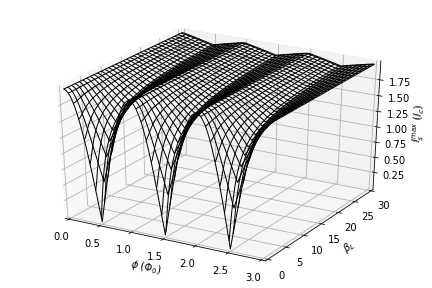
\includegraphics[width=0.5\linewidth]{./chapter-theory/figs-JJ/SQUID_betaL}
	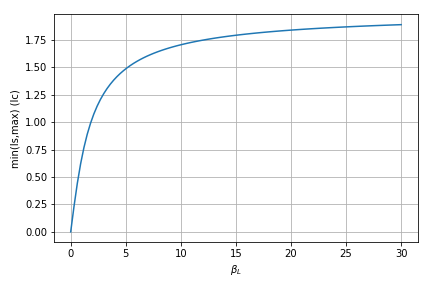
\includegraphics[width=0.4\linewidth]{./chapter-theory/figs-JJ/SQUID_betaL_I}
	\caption{Critical current modulation of SQUID for various screening factors $\beta_L$.}
	\label{fig:betaL}
\end{figure}

\section{Induced superconductivity and Josephson junctions}

\dropcap{T}{he} process of Andreev reflection at the interface between superconductors and normal metals lays the fundament for understanding how a Josephson junction works.
The process is sketched in Fig. \ref{fig:kdtmk}:
An electron impinging onto the super-normal interface from inside the normal region can only enter the superconductor in the form of a Cooper pair by being reflected as a hole with opposite spin and momentum.
Vice versa, a Cooper pair travelling towards the normal region will decay into an electron travelling forward, and annihilate a hole travelling backwards with spin opposite to that of the electron.
Inside the normal region, this will result in the formation of the so-called Andreev bound states (ABS).

\begin{figure}
	\centering
	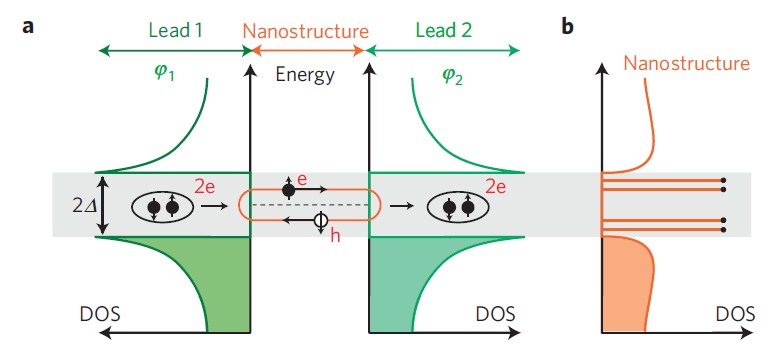
\includegraphics[width=0.7\linewidth]{./chapter-theory/figs-JJ/KDTMK}
	\caption{The formation of Andreev bound states inside of a Josephson junction due to Andreev reflection at the SN interface.}
	\label{fig:kdtmk}
\end{figure}

Since inside the superconductor, there are no states allowed for $\epsilon_F - \Delta \leq \epsilon_F \leq \epsilon_F - \Delta$, the superconducting electrodes can be though of as forming potential barriers at the interface, leading to transparencies $\tau$, and the Andreev paris can be thought of analogously as particles inside a box.
Here also elaborate on the Thouless energy and 2D junctions.

The energy of these particles is given by
%
\begin{eqnarray}
E_{\pm}(\delta,\tau)=\pm\Delta\sqrt{1-\tau\sin^2(\delta/2)},
\end{eqnarray}
%
with each Andreev state ($\pm$) carrying a supercurrent
%
\begin{eqnarray}
I_{\pm}(\delta,\tau)=\frac{1}{\Phi_0}\diffp{ E_{\pm}(\delta,\tau)}{\delta}=\mp\frac{\Delta}{4\Phi_0}\frac{\tau\sin(\delta)}{\sqrt{1-\tau\sin^2(\delta/2)}}
\label{eq:CPR-full}
\end{eqnarray}

For temperature $T\rightarrow0$, all states with $E<\epsilon_F$ are unoccupied, so only the lower-lying Andreev state $E_{-}(\delta)$ carries current.
%
The critical current of the junction is given by the maximum current possible being carried by the state. Mathematically, this equals
%
\begin{eqnarray}
I_c=\max_\delta I_{-}(\delta) \Rightarrow \diff{I_{-}(\delta)}{\delta}\equiv0=-\Delta\tau\frac{-4(\tau-2)\cos(\delta)+\tau(3+\cos(2\delta))}{8\sqrt{2}\Phi_0(2-\tau+\tau\cos(\delta))^{3/2}}
\label{eq:ABS-start}
\end{eqnarray}

After a lot of math (see Appendix \ref{app:eqs}), we arrive at a compact expression for the critical current of a single ABS channel,
%
\begin{eqnarray}
I_c = \frac{\Delta}{2\Phi_0}\left( 1-\sqrt{1-\tau} \right).
\label{eq:ABS-stop}
\end{eqnarray}

For finite temperatures, also electronic states above the gap are filled according to the Fermi-Dirac distribution
\begin{align}
f(T,x)=\frac{1}{1+e^{x/k_BT}} \ ,
\label{eq:fermidirac}
\end{align}
with the Boltzmann constant $k_B$.
%
The total current of an ABS pair traversing the JJ is consequently
\begin{align}
I_J(\delta,\tau,T) &= \sum_n \left[ I_+\left(\delta,\tau\right) f\left(T,E_+\left(\delta,\tau\right)\right) + I_-\left(\delta,\tau\right) f\left(T,E_-\left(\delta,\tau\right)\right) \right] \\
&=\frac{\pi\Delta_0}{2 e R_n} \frac{\sin\delta}{\sqrt{1 - \tau \sin^2\delta / 2}} \tanh\left[\frac{\Delta_0}{k_B T} \sqrt{1 - \tau \sin^2\delta / 2}\right]\ ,
\label{eq:CPR-ball}
\end{align}



\subsection{SIS junctions: $\tau \rightarrow 0$}
If the weak link between the superconducting banks is an insulator, we can take eq.\ref{eq:ABS-stop} in the limit $\tau \rightarrow 0$ to arrive at\footnote{$\sqrt{1-\tau x}\approx 1-\tau x/2+\mathcal{O}(\tau x)^2\rightarrow 1$.}

\begin{eqnarray}
I(\delta)=\frac{\Delta\tau}{4\Phi_0}\sin(\delta),
\end{eqnarray}

for each Andreev channel. The overall junction critical current for $N$ channels is then 
\begin{eqnarray}
	I_c=\frac{\Delta}{4\Phi_0}\sum_{i}^{N_i}\tau_i
\end{eqnarray}

\textcolor{red}{\textbf{Note:} I think it might be more useful to do a short recap of Golubov, Kupriyanov and Il'ichev 2004. 
They start from the general cases of current-phase relations and develop from there.
Relevant cases for us are KO-1, point-contact, tunnel junctions and clean and dirty SNS ones.}

\subsection{Current bias}

The washboard potential is 
%
\begin{align}
U(\delta) = -E_J \left( \cos\delta + \frac{I_b}{I_c}\delta \right)
\label{eq:washboard}
\end{align}

\subsection{Voltage bias}
Voltage biasing a Josephson junction leads to a process called Multiple Andreev reflection (MAR).
We did measurements on this of our graphene Josephson junctions.
It is important to note, that the voltage measured across a DC current-biased Josephson junction is not a pure DC voltage, but rather the time-averaged value of the oscillating $V=\partial\delta/\partial t$.
This effectively leads to the emission of Josephson radiation from the junction, with the frequency being tuned via the bias voltage.
This phenomenon can be controlled so precise, that it serves as the definition of the voltage standard nowadays.
A plethora of potential applications of Josephson radiation in cicruit electrodynamics have been proposed and realized (such as the Josephson laser).
However, the realization of such devices needs to be engineered quite precise, as reaching oscillation frequencies in the GHz regime requires bias voltages in the microvolt range, often requiring small shunt resistors which pull the Josephson junction far into the overdamped regime.